\documentclass{beamer}
\usepackage{color,amsmath,comment, subfigure}
\usepackage{booktabs}
\def\vf{\vfill}
\usepackage{url}

%\setbeameroption{show notes}

%%%%%%%%%%%%%%%%%%%%%%%%%%
\title[]{Lecture 6: Foci}
\author[]{Matthew Salganik}
\institute[]{Sociology 204: Social Networks, Spring 2021\\Princeton University}
\date[]{
1/3: Lois Weisberg and social structure

\vfill

\begin{flushleft}
\vspace{0.7in}

\includegraphics[width=0.05\textwidth]{figures/cc.png}
\end{flushleft}
}

\begin{document}
%%%%%%%%%%%%%%%%%%%%%%%%%%%
\frame{\titlepage}
%%%%%%%%%%%%%%%%%%%%%%%%%%%
\begin{comment}
\begin{frame}

SWBAT:
\begin{enumerate}
\item realize the power of edges that don't exist
\item compare psychological vs sociological explanations for network structure
\item apply the idea of foci to understand their personal networks 
\item see how sociological principles can shape the design of technical systems
\end{enumerate}

\end{frame}
\end{comment}
%%%%%%%%%%%%%%%%%%%%%%%%
\begin{frame}
\frametitle{Review}

\begin{itemize}
\item growth + preferential attachment $\rightarrow$ power law degree distribution
\pause
\item some (but not all) real networks have a power law degree distribution 
\pause
\item diseases spread more easily on networks with power law degree distribution than on other types of networks
\pause
\item networks with power law degree distribution are robust to random failure but fragile to targeted attack
\pause
\item ``hubs'' seem important
\end{itemize}

\end{frame}
%%%%%%%%%%%%%%%%%%%%%%%
\begin{frame}

\begin{figure}
  \centering
  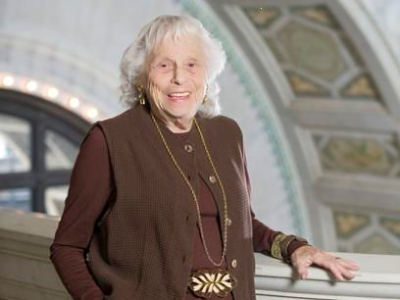
\includegraphics[width=0.8\textwidth]{figures/lois_weisberg}
\end{figure}

Her story connects 2 ideas: power law degree distributions and foci
\vfill

\tiny{Source: \url{www.wbez.org}}

\note{
Lois Weisberg is a ``connector'' (something Gladwell talks about more in tipping point).  For our purposes Lois also connects two ideas: power law degree distributions and foci.  ``It is not nearly that she knows lots of people.  It is that she belongs to lots of different worlds.''  Lois belonged to eight worlds: the actors, the writers, the doctors, the lawyers, the park lovers, the politicians, the railroad bugs, and the flea-market aficionados.  Thus it is not just her ties, but the lack of ties between her friends.  In other words we have talked about ties, now we are going to talk about lack of ties.
}

\end{frame}
%%%%%%%%%%%%%%%%%%%%%%%%%%%%
\begin{frame}

``It is not nearly that she knows lots of people.  It is that she belongs to lots of different worlds.'' 
\pause
\begin{itemize}
\item the actors
\pause
\item the writers
\pause
\item the doctors
\pause
\item the lawyers
\pause
\item the park lovers
\pause
\item the politicians
\pause
\item the railroad bugs
\pause
\item the flea-market aficionados
\end{itemize}

\pause
\vfill
A key point is that these people don't know each other. That enables Lois to be a ``broker''.
\note{
Not just her connections but the lack of connections between people she knows
}

\end{frame}
%%%%%%%%%%%%%%%%%%%%%%%%%%%%
\begin{frame}

\begin{figure}
  \centering
  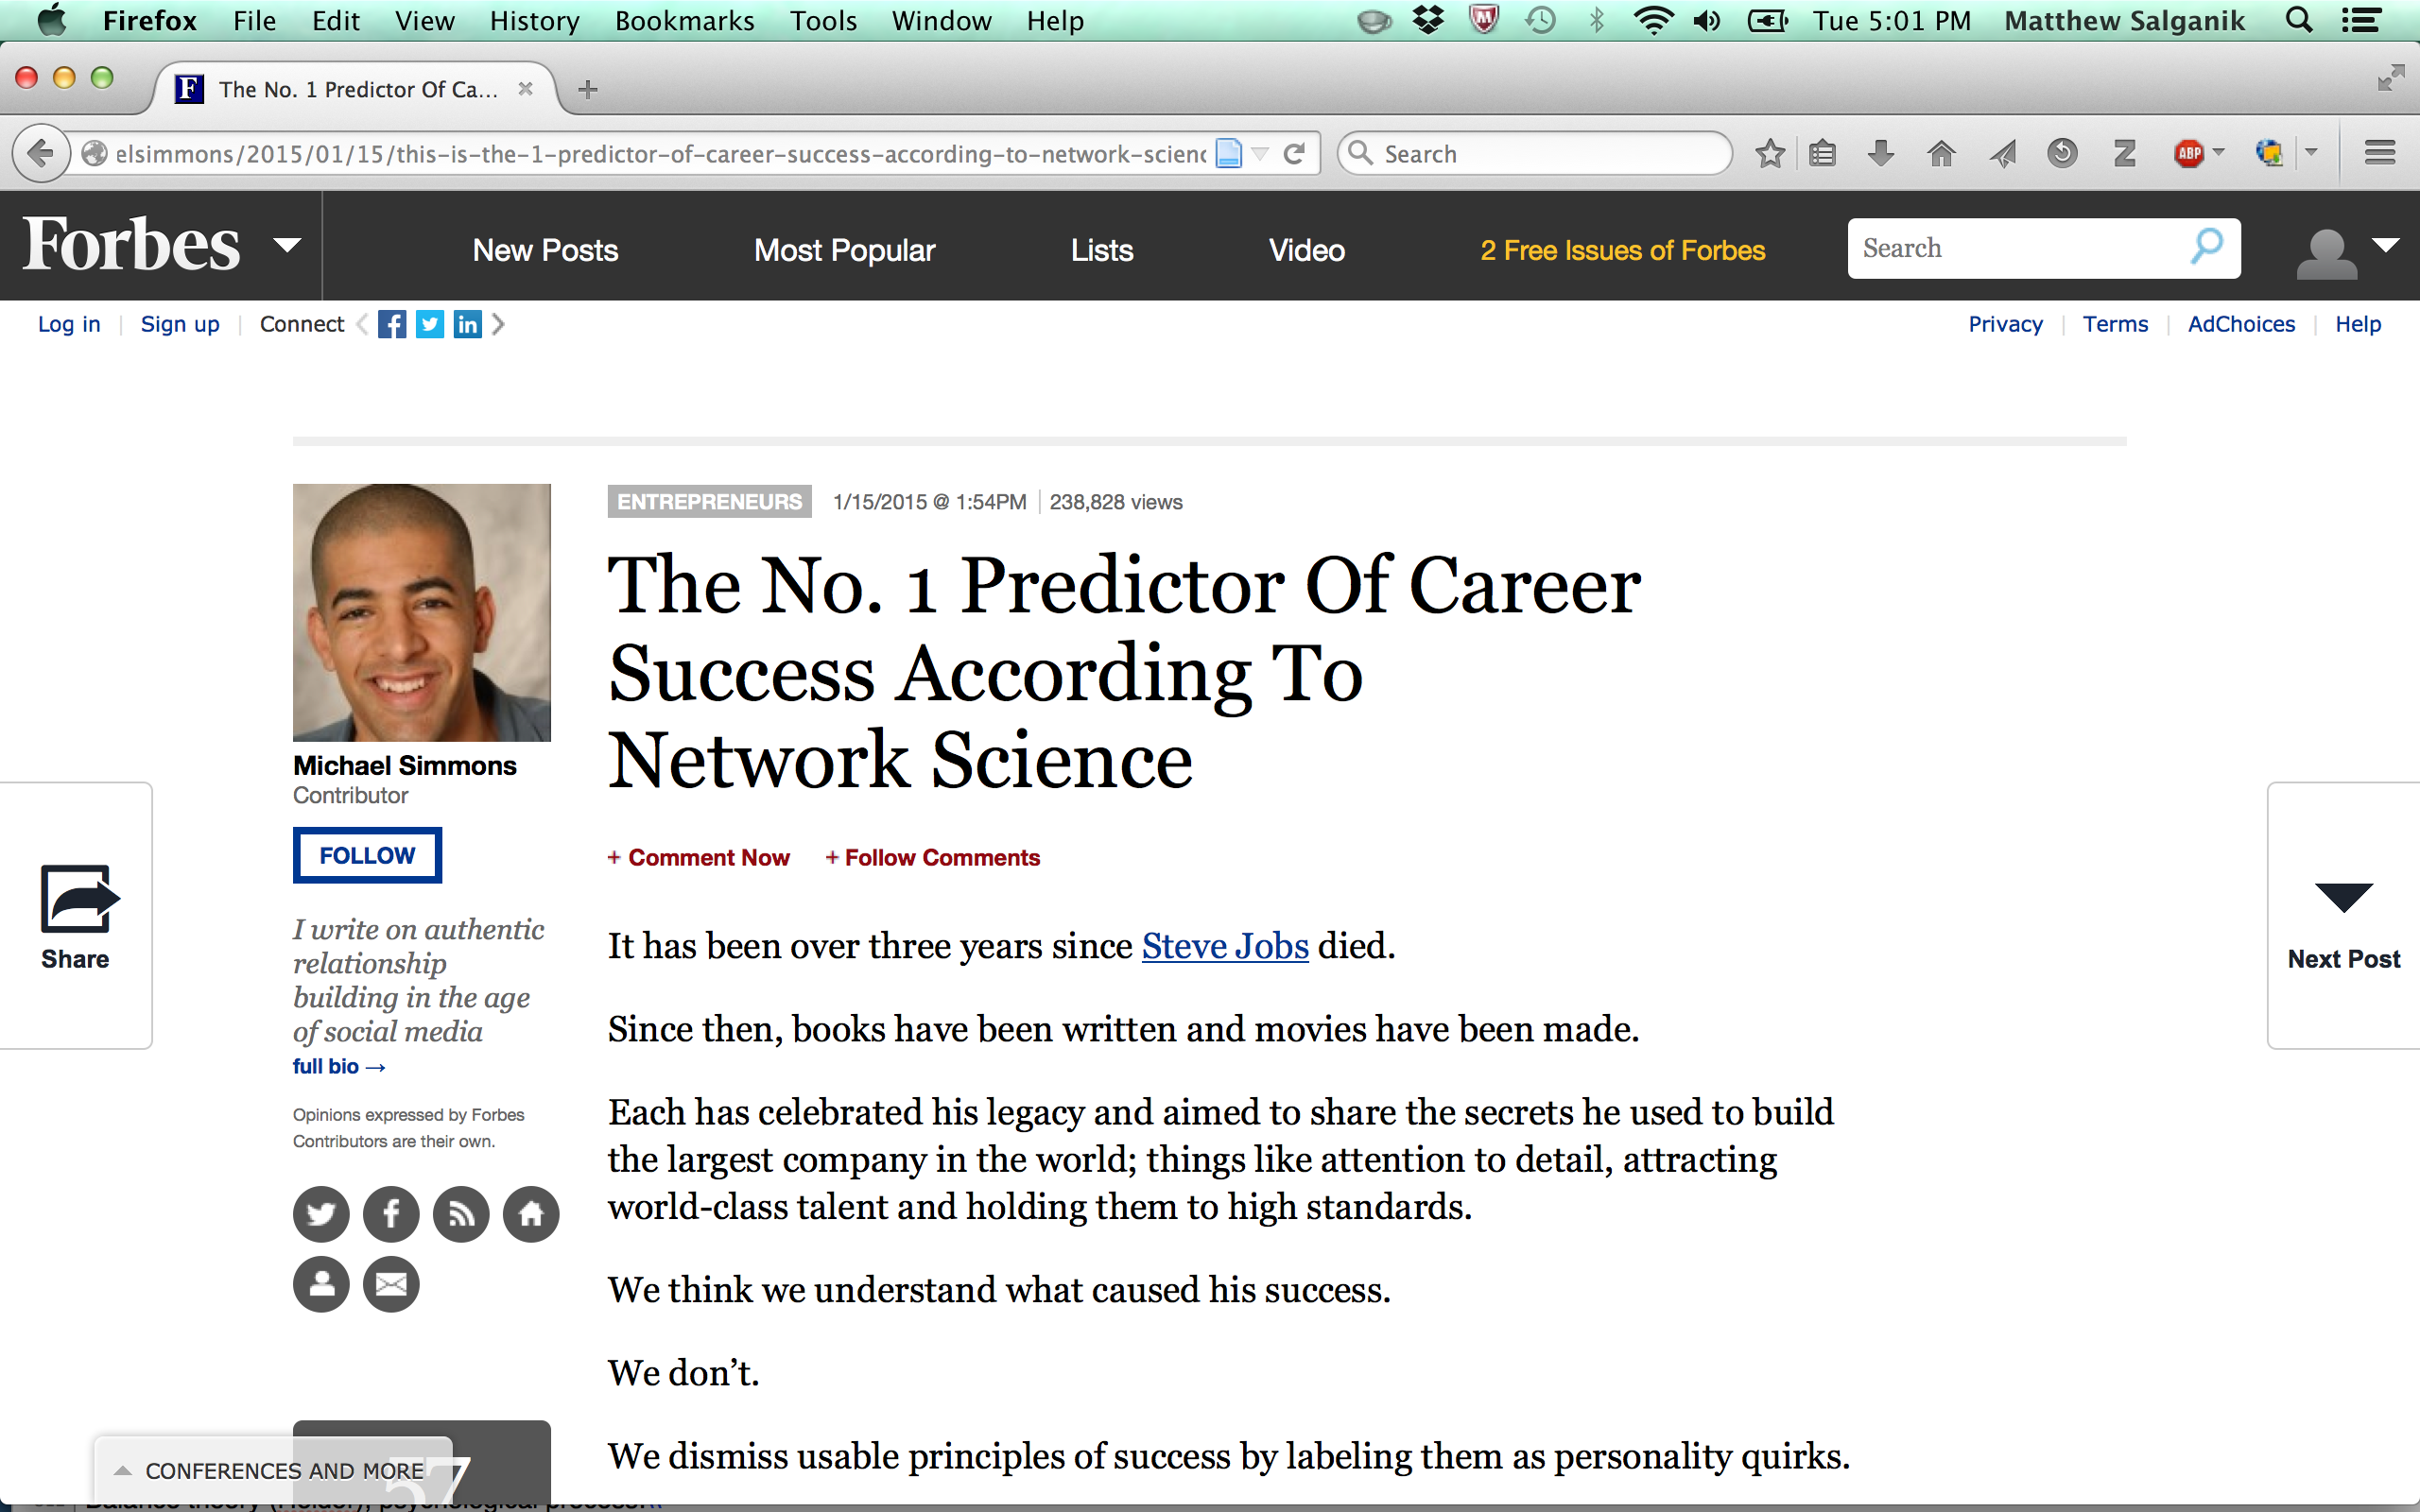
\includegraphics[width=0.9\textwidth]{figures/simmons_predictor_2015}
\end{figure}

\tiny{Source: \url{http://www.forbes.com/sites/michaelsimmons/2015/01/15/this-is-the-1-predictor-of-career-success-according-to-network-science/}}

\note{open networks are good in firms}

\end{frame}
%%%%%%%%%%%%%%%%%%%%%%%%%%%%
\begin{frame}

\begin{figure}
  \centering
  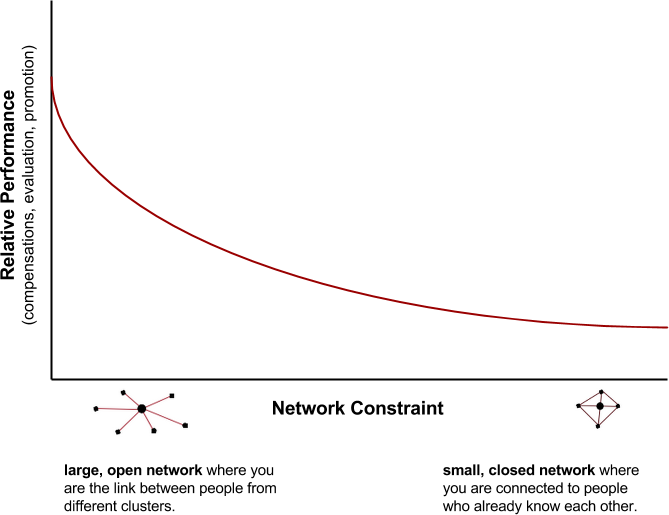
\includegraphics[width=0.9\textwidth]{figures/Burt_Success_Final.png}
\end{figure}

\tiny{Source: \url{http://www.forbes.com/sites/michaelsimmons/2015/01/15/this-is-the-1-predictor-of-career-success-according-to-network-science/}}

\note{open networks are good in firms}

\end{frame}
%%%%%%%%%%%%%%%%%%%%%%%%%%%%
\begin{frame}

\begin{figure}
  \centering
  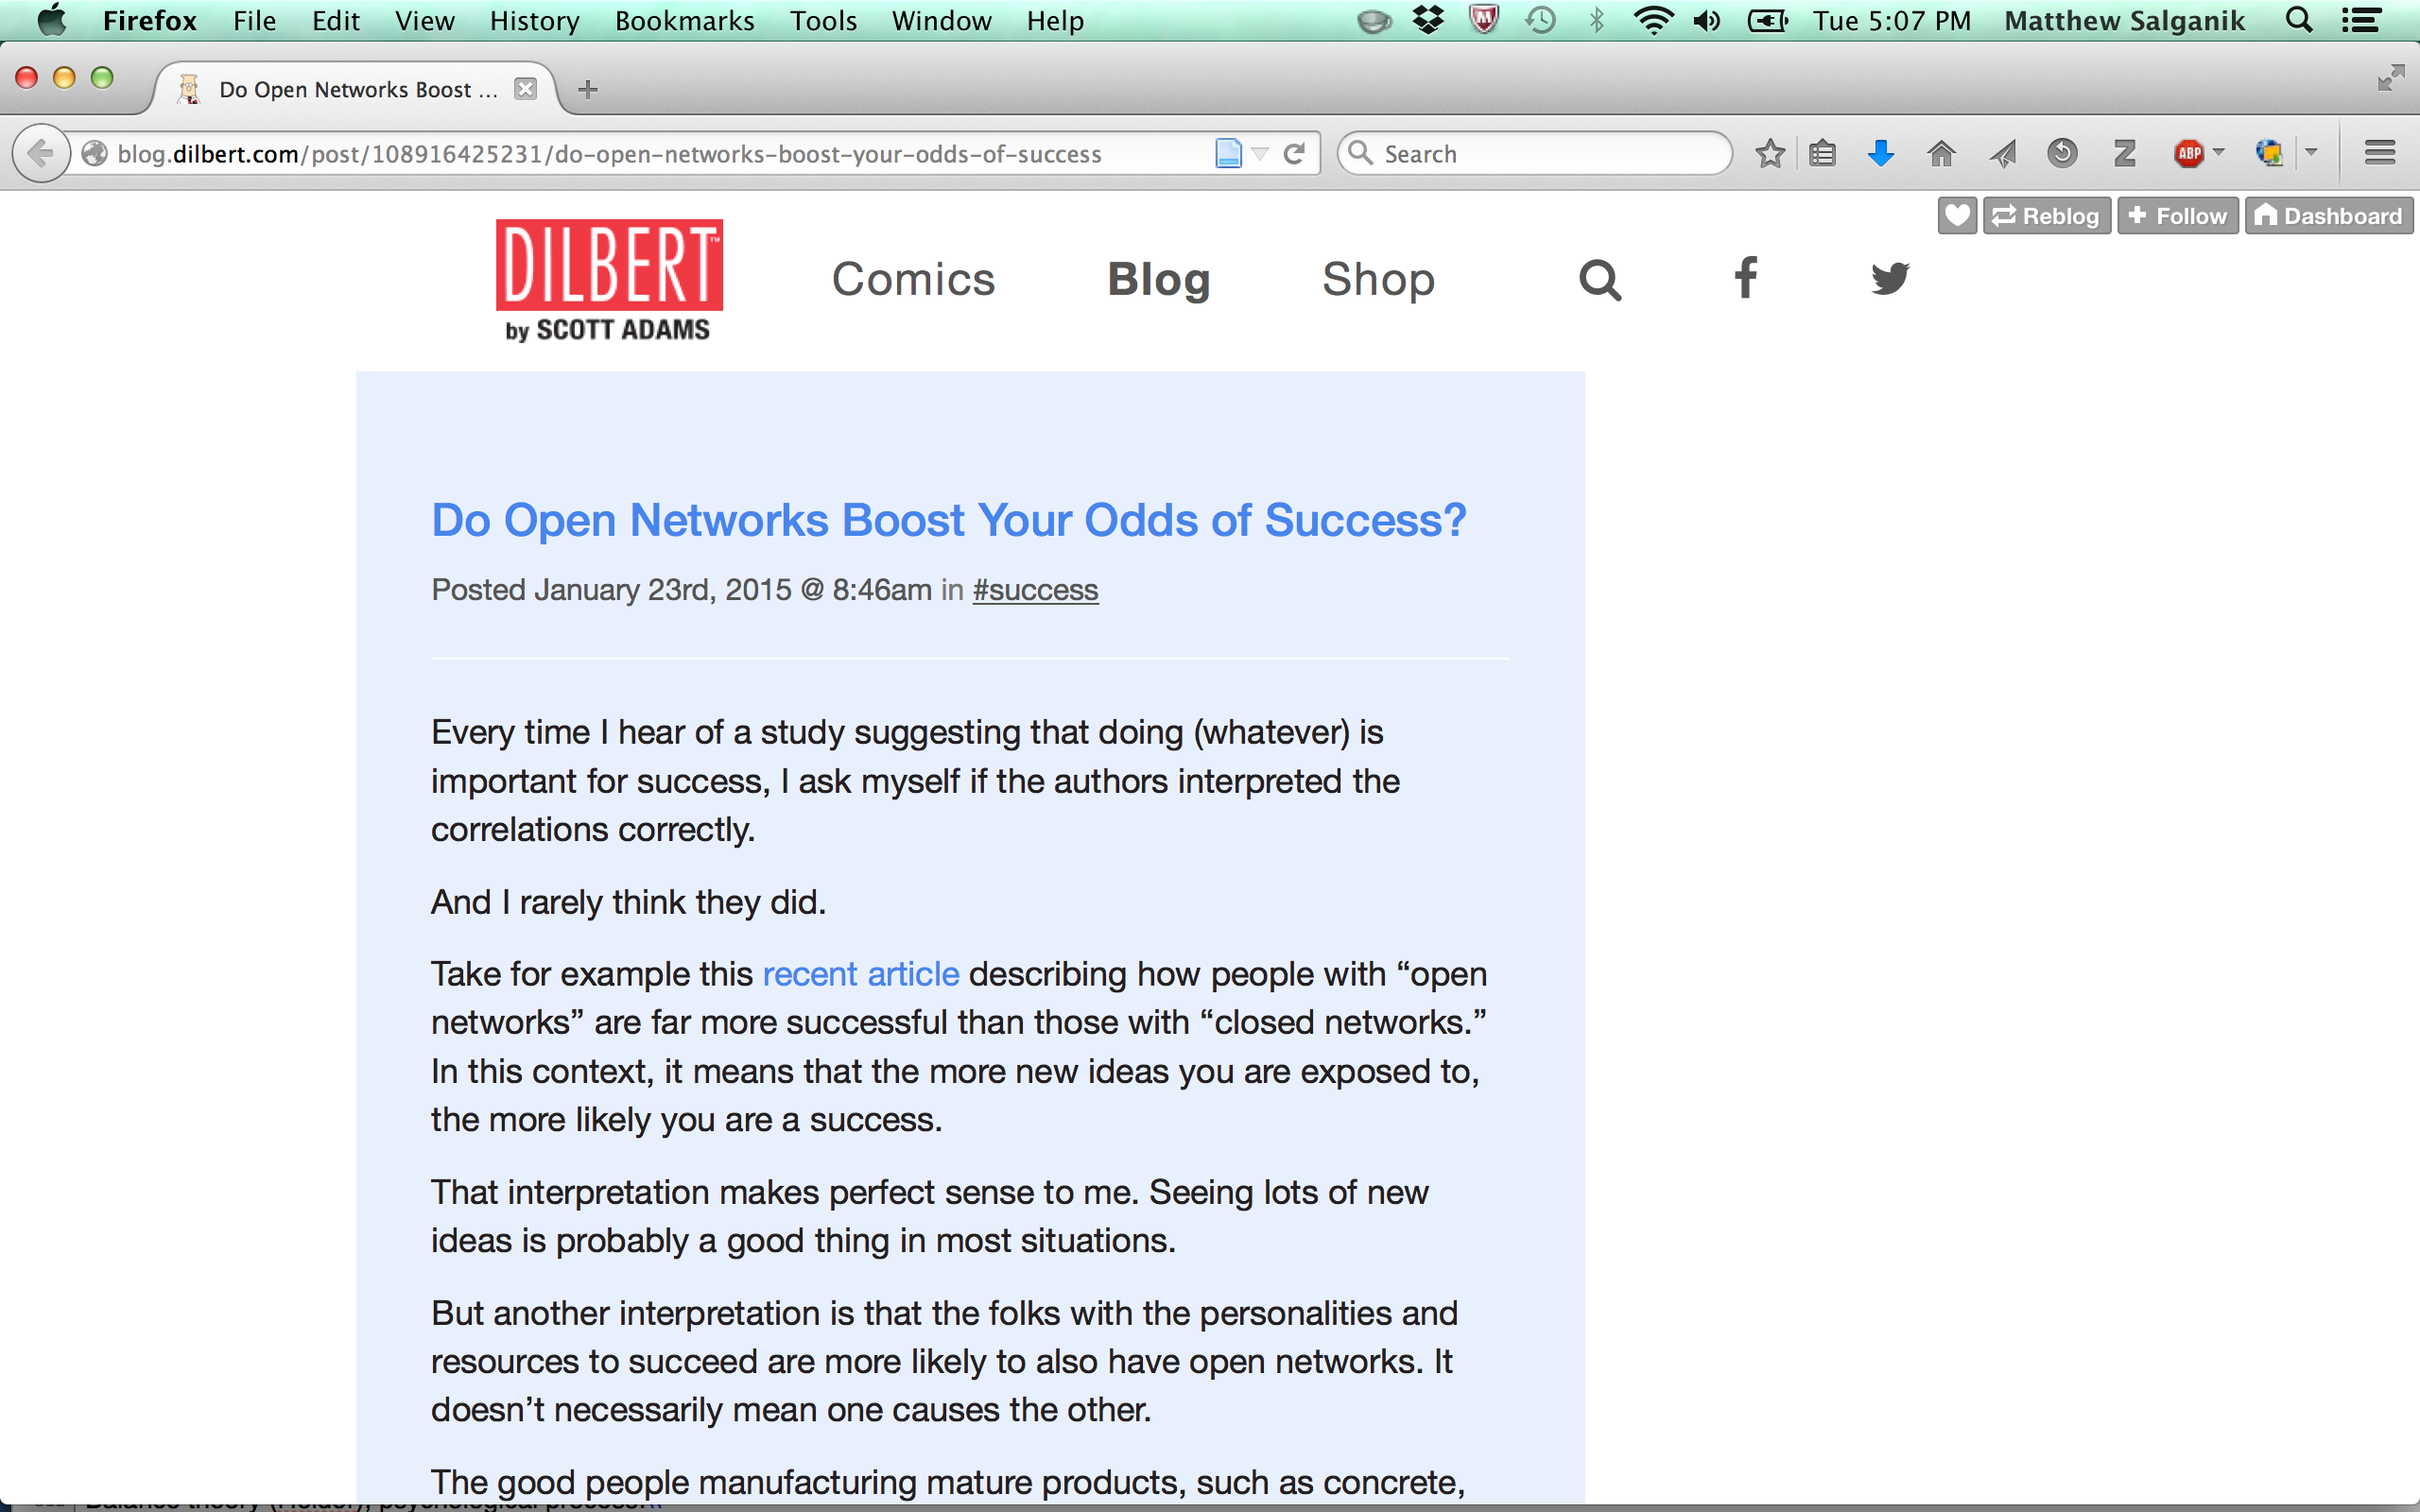
\includegraphics[width=0.9\textwidth]{figures/adams_do_2015}
\end{figure}

\tiny{Source: \url{http://blog.dilbert.com/post/108916425231/do-open-networks-boost-your-odds-of-success}}

\note{correlation is not causation}

\end{frame}
%%%%%%%%%%%%%%%%%%%%%%%%%%%%
\begin{frame}

\begin{figure}
  \centering
  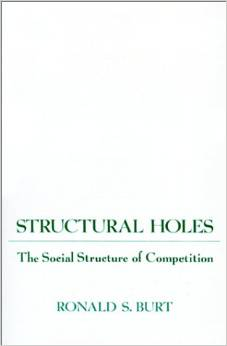
\includegraphics[height=0.8\textheight]{figures/burt_structural_1995}
\end{figure}

\note{For the real details see Burt}

\end{frame}
%%%%%%%%%%%%%%%%%%%%%%%%%%%
\begin{frame}

How does Lois Weisberg's story---and the readings more generally---change how we should think about networks?

\pause 

Combines:
\begin{itemize}
\item network structure
\item social structure 
\end{itemize}

\note{
What is social structure?  For our purposes groups.
}

\end{frame}
%%%%%%%%%%%%%%%%%%%%%%%%%%%
% 2/2 Social structure
%%%%%%%%%%%%%%%%%%%%%%%%%%%
\begin{frame}

Affiliation network
\begin{figure}
  \centering
  \includegraphics[width=0.75\textwidth]{figures_book/4_6_bi.png}
\end{figure}
\pause
\begin{itemize}
\item actors and movies
\pause
\item scientists and papers
\pause
\item board members and boards of directors
\end{itemize}

\note{
Looking only at the network of relationships, you can get confused.  The real driver is the combination of people and foci.

Feld work helps us think about foci, overlap of foci, and how they create ties.
}

\end{frame}
%%%%%%%%%%%%%%%%%%%%%%%%%%
\begin{frame}

\begin{figure}
  \centering
  \includegraphics[width=0.75\textwidth]{figures_book/4_6_bi_group.png}
\end{figure}

\end{frame}
%%%%%%%%%%%%%%%%%%%%%%%%%%
\begin{frame}

\begin{figure}
  \centering
  \includegraphics[width=0.75\textwidth]{figures_book/4_6_bi_actor.png}
\end{figure}

\end{frame}
%%%%%%%%%%%%%%%%%%%%%%%%%%
\begin{frame}

\begin{figure}
  \centering
  
\includegraphics[width=0.8\textwidth]{figures/feld_focused_1981_title}
\end{figure}

\pause

\begin{itemize}
\item you are stepping in a conversation
\pause
\item a very dense---but interesting---conversation
\end{itemize}

\end{frame}
%%%%%%%%%%%%%%%%%%%%%%%%%%%
\begin{frame}

Foci: a social, psychological, or physical entity around which joint activities are organized. 

\end{frame}
%%%%%%%%%%%%%%%%%%%%%%%%%%%
\begin{frame}

\begin{center}
 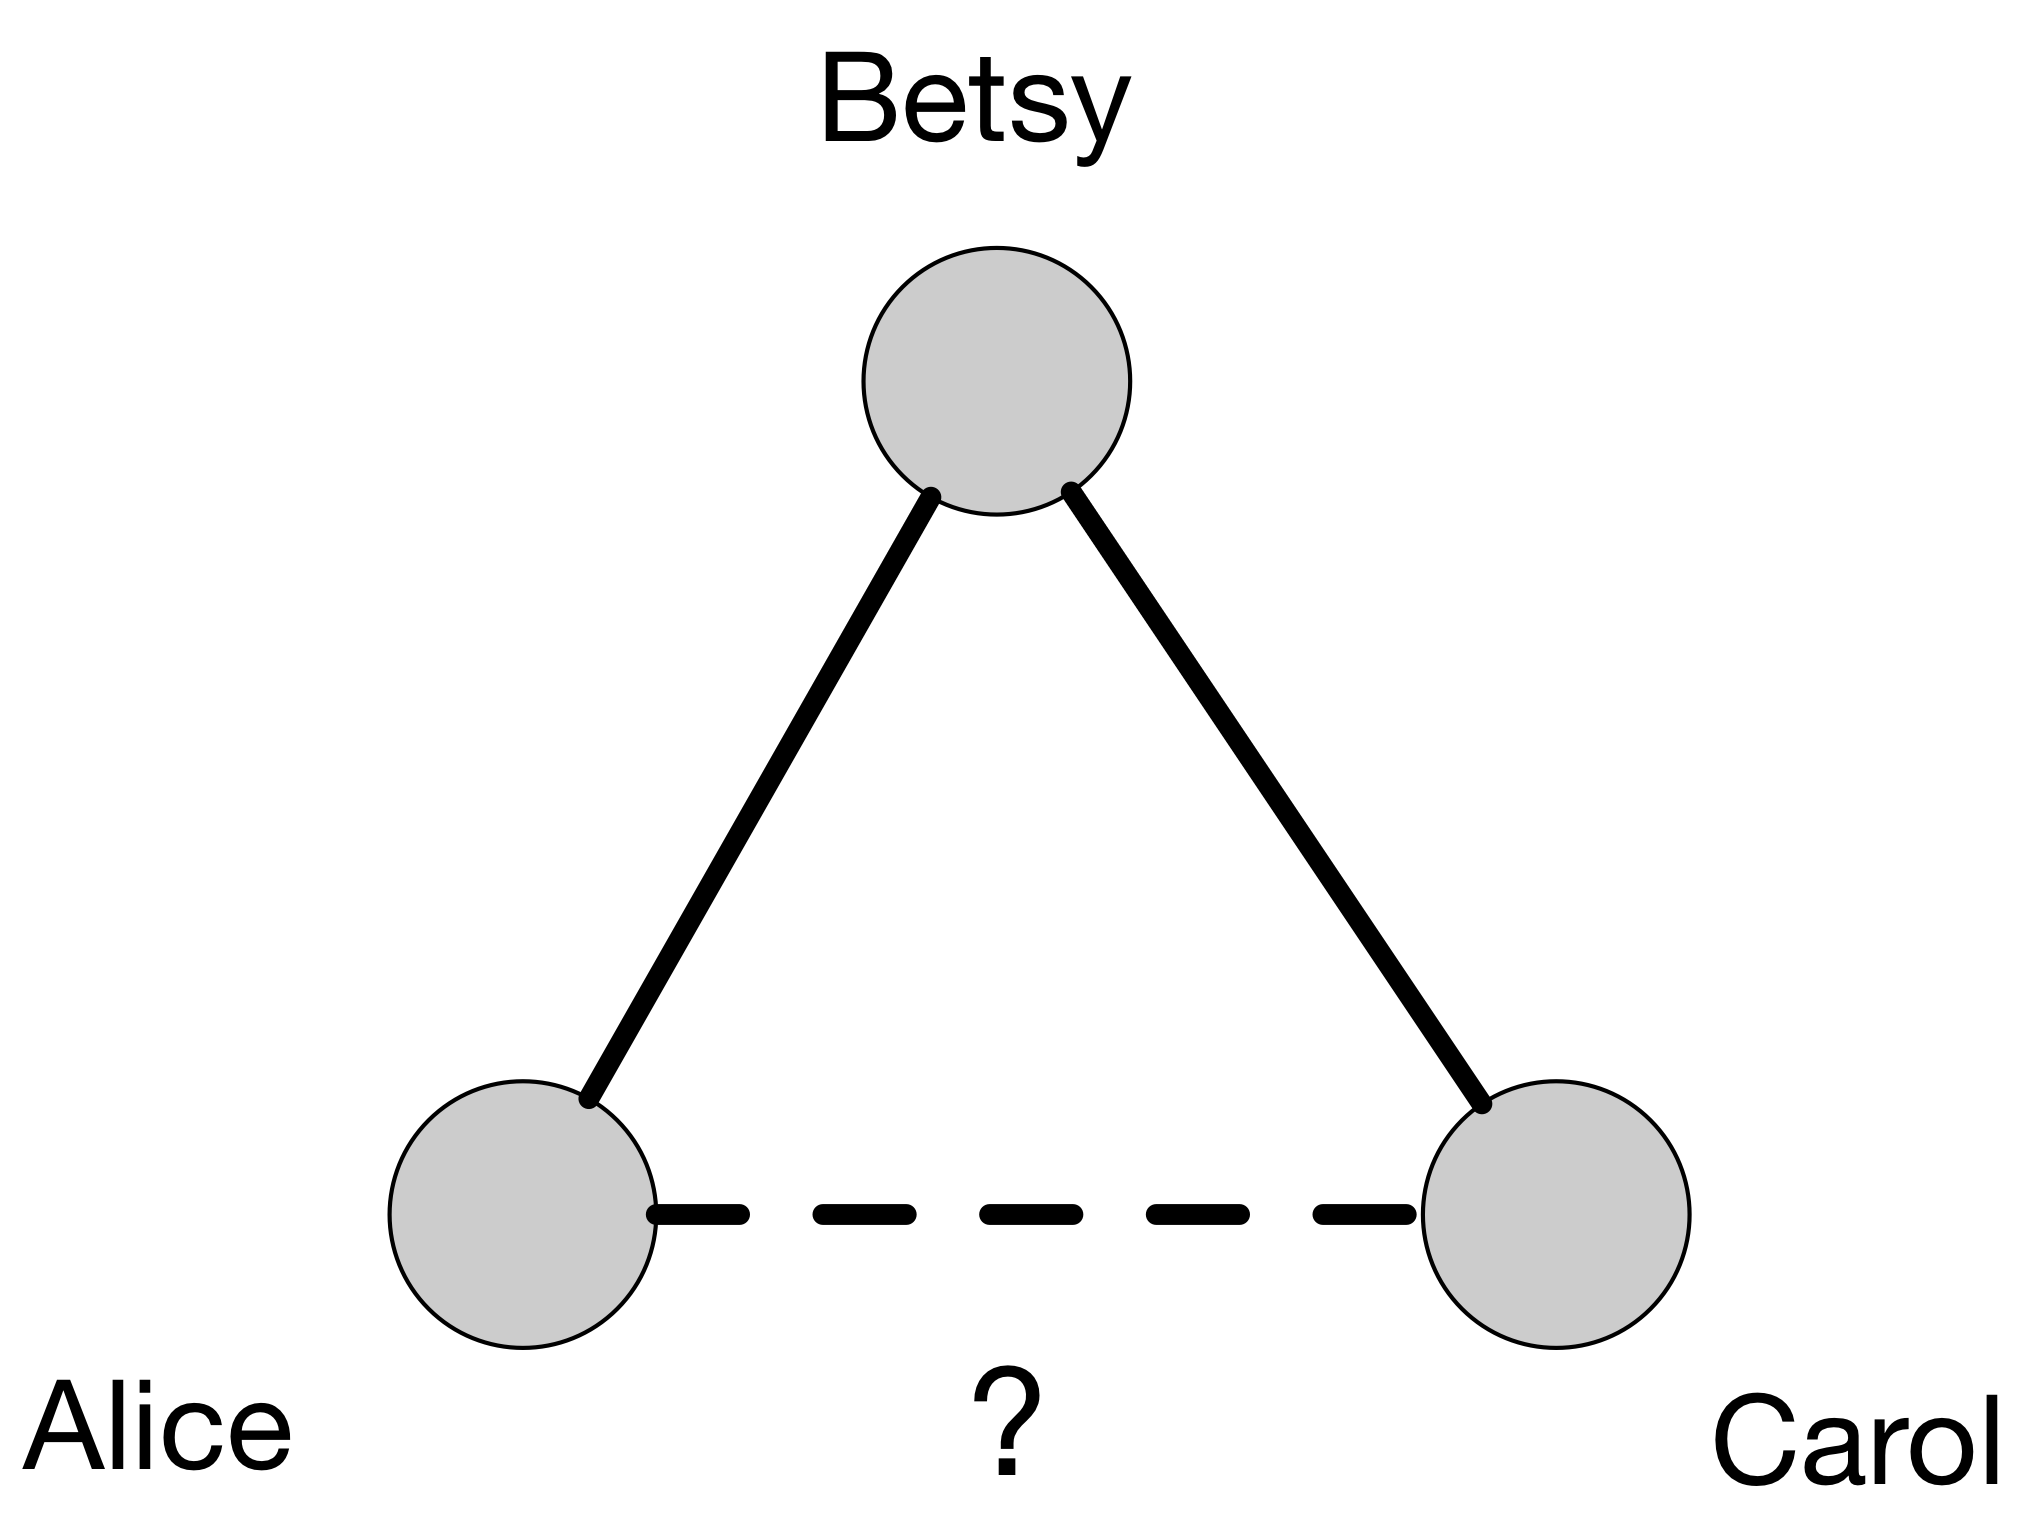
\includegraphics[width=0.6\textwidth]{figures/triadic_closure}
\end{center}

Explaining triadic closure:
\begin{itemize}
\item balance theory vs foci
\item psychology vs sociology
\item agency vs structure
\end{itemize}

\note{
This contrast is clear in Feld when he compares foci to balance theory. 
Balance theory (Heider), psychological process:\\
If Alice likes Betsy and Betsy likes Carol then Alice should like Carol to bring their relationship into to ``balance''\\
Feld said no.  Social structure not psychology\\
This is an example of more broader shift in the way to think about the world sociology over psychology, structure over agency
}

\end{frame}
%%%%%%%%%%%%%%%%%%%%%%%%%%%
\begin{frame}

\begin{center}
{\Large Roughly speaking: you don't pick your friends, your environment picks your friends for you}
\end{center}

\end{frame}
%%%%%%%%%%%%%%%%%%%%%%%%%%%%
\begin{frame}

\begin{center}
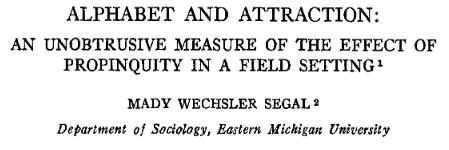
\includegraphics[width=0.95\textwidth]{figures/segal_alphabet_1974_title}
\end{center}

\vfill
\url{http://dx.doi.org/10.1037/h0037446}

\end{frame}
%%%%%%%%%%%%%%%%%%%%%%%%%%%%
\begin{frame}

\begin{center}
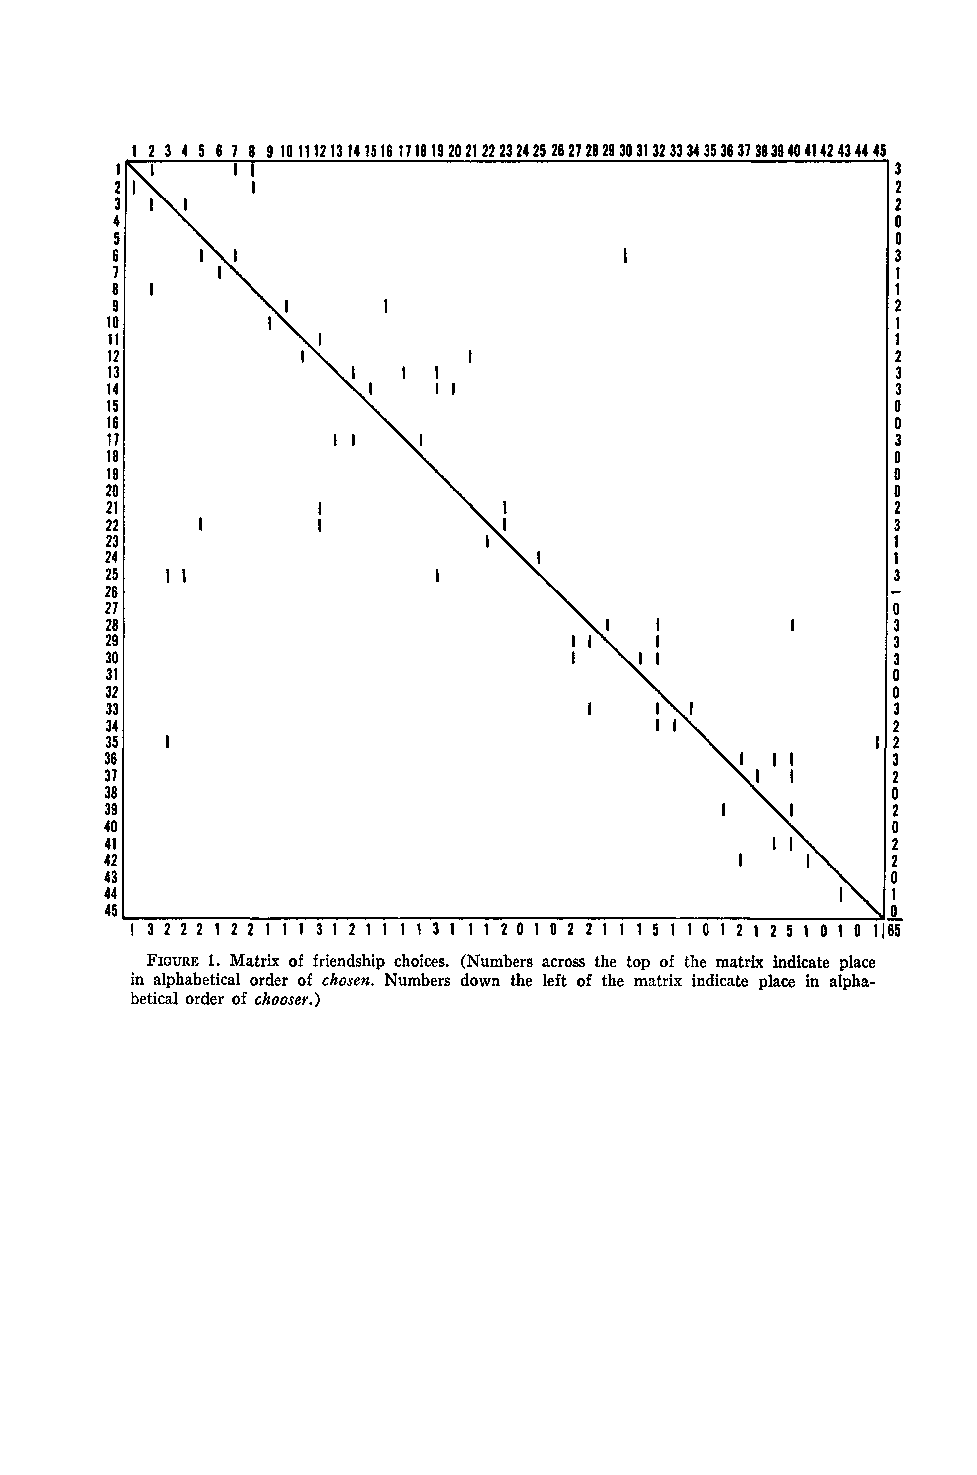
\includegraphics[width=0.8\textwidth]{figures/segal_alphabet_1974_fig1}
\end{center}

\end{frame}
%%%%%%%%%%%%%%%%%%%%%%%%%%%%
\begin{frame}

\begin{center}
 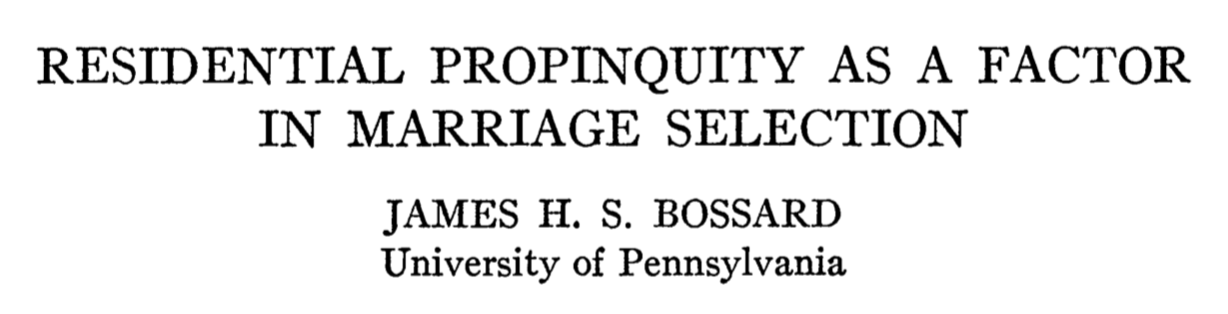
\includegraphics[width=0.8\textwidth]{figures/bossard_residential_1932_title}
\end{center}

\begin{itemize}
\item study of 5,000 marriage licenses in which one or both applicant lived in Philadelphia (January - May 1931)
\end{itemize}

\vfill
\url{https://www.jstor.org/stable/2766455 }

\end{frame}
%%%%%%%%%%%%%%%%%%%%%%%%%%%
\begin{frame}

\begin{center}
 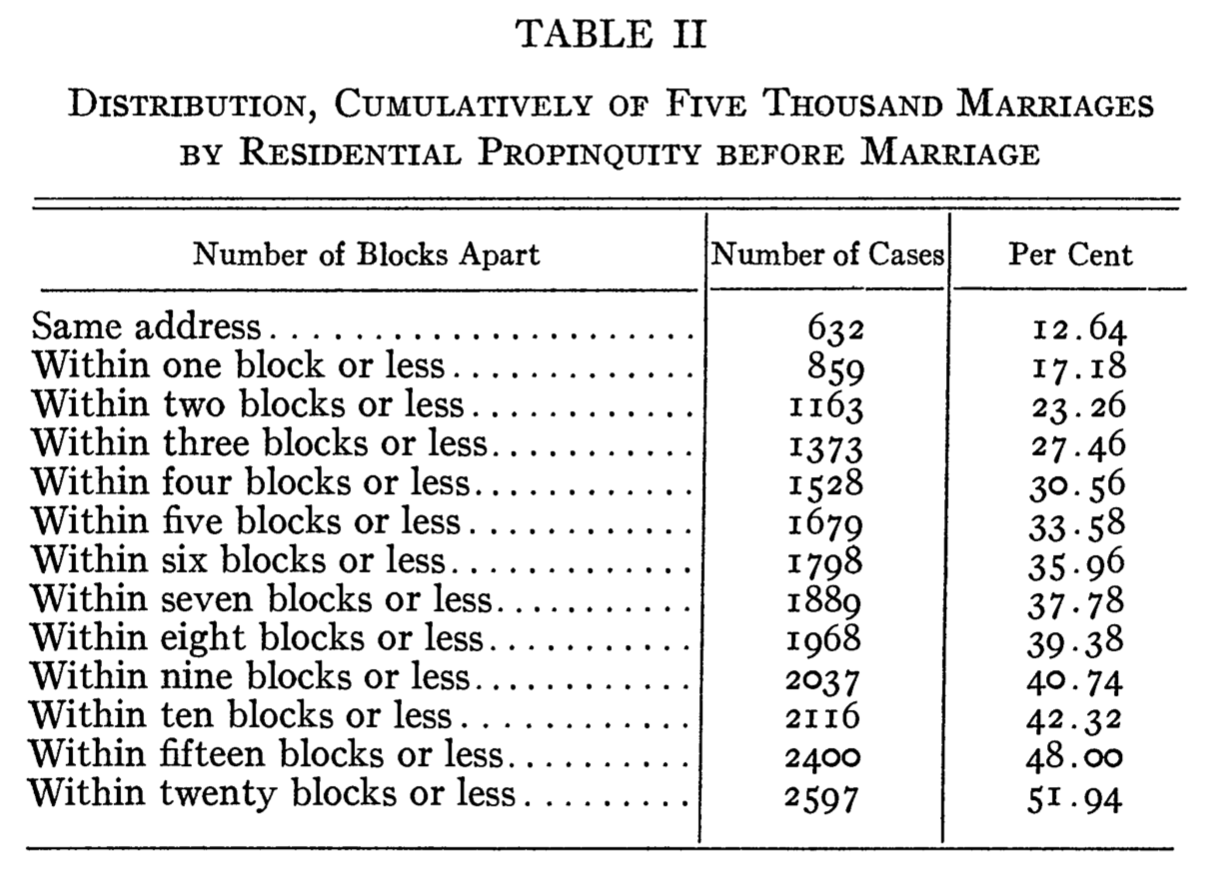
\includegraphics[height=0.7\textheight]{figures/bossard_residential_1932_tab2}
\end{center}

\begin{itemize}
\item More than one in three couples involved a person lived within 5 blocks or less. 
\pause
\item Bossard (1932): ``Cupid may have wings, but apparently they are not adapted for long flights.''
\end{itemize}

\note{
Things not as extreme as in 1932 but geography still plays a huge role in the formational of relationships
}

\end{frame}
%%%%%%%%%%%%%%%%%%%%%%%%%%%
\begin{frame}

\begin{itemize}
\item The theory of foci calls attention to the fact that many network ties are formed because of social structure.
\pause
\item What do foci have to do with Facebook and Google+?
\end{itemize}

\end{frame}
%%%%%%%%%%%%%%%%%%%%%%%%%%%
% 3/3 Foci in the design of technical systems
%%%%%%%%%%%%%%%%%%%%%%%%%%%
\begin{frame}

\begin{center}
 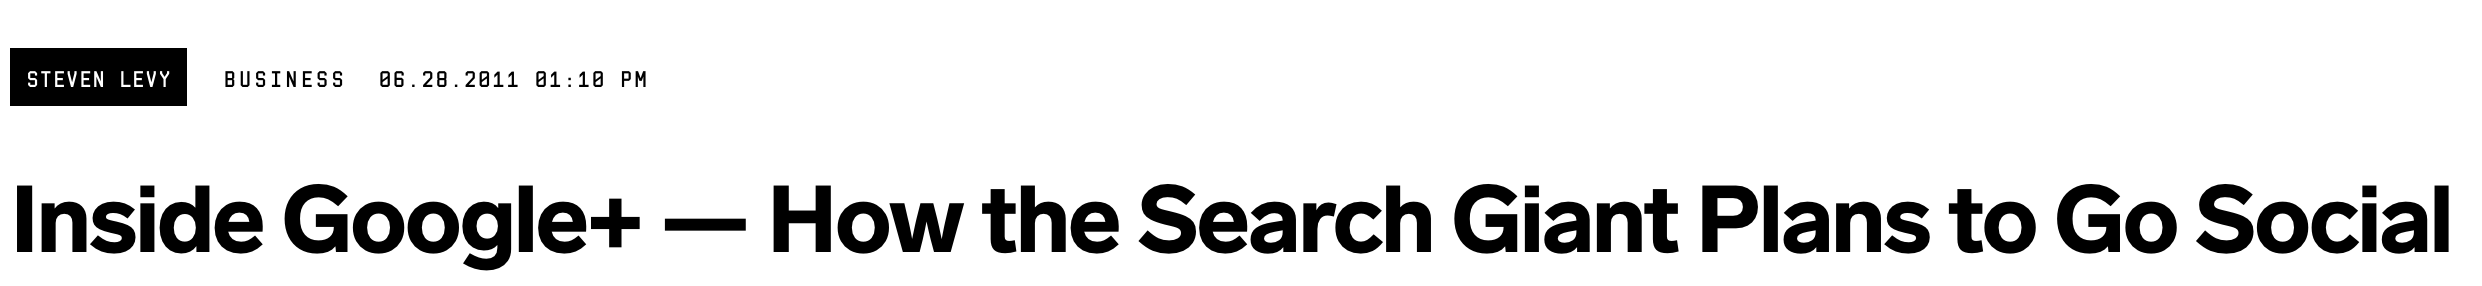
\includegraphics[height=0.7\textheight]{figures/levy_inside_2011_title}
\end{center}

\vfill

\url{https://www.wired.com/2011/06/inside-google-plus-social/}

\end{frame}
%%%%%%%%%%%%%%%%%%%%%%%%%%
\begin{frame}


\begin{center}
 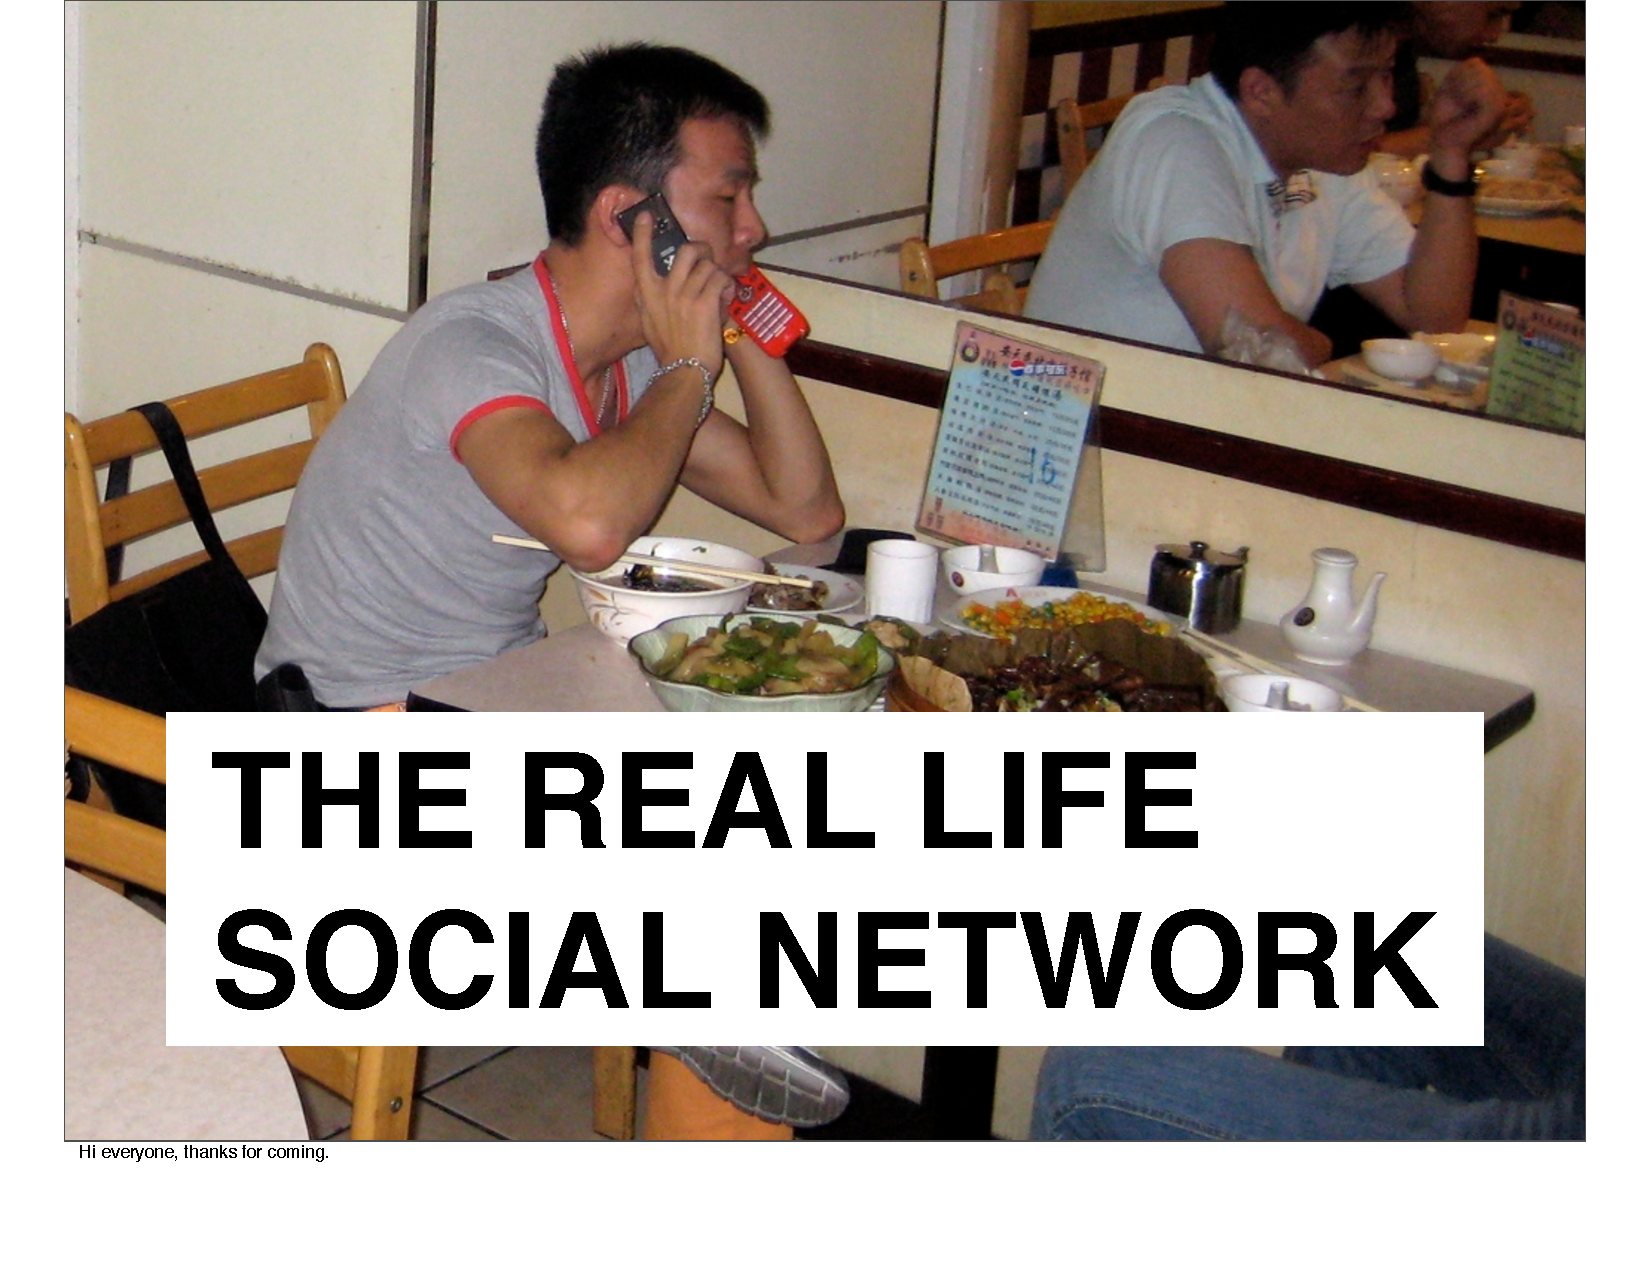
\includegraphics[width=0.7\textwidth]{figures/adams_real_2011_page1}
\end{center}

\vfill
\url{https://www.businessinsider.com/heres-the-presentation-that-inspired-google-2011-7}

\end{frame}
%%%%%%%%%%%%%%%%%%%%%%%%%%
\begin{frame}

More about Google Plus:
\begin{itemize}
\item Paul Adams \textit{Grouped: How Small Groups of Friends are the Key to Influence on the Social Web}
\item ``Google Plus: a \$585 million dollar mistake'': \url{https://slidebean.com/blog/startups-google-plus}
\item ``Looking back at Google+'': \url{https://techcrunch.com/2018/10/08/looking-back-at-google/}
\item \url{https://en.wikipedia.org/wiki/Google\%2B}
\end{itemize}

\end{frame}
%%%%%%%%%%%%%%%%%%%%%%%%%
\begin{frame}

\begin{itemize}
\item sometimes the edges that don't exist are as important as the edges that do exist
\pause
\item affiliation networks (people and groups) help us understand patterns in personal network structure
\pause
\item compare and contrast psychological vs sociological explanations for network structure 
\pause
\item sociological principles can shape the design of technical systems
\end{itemize}

\end{frame}
%%%%%%%%%%%%%%%%%%%%%%%%%%%
\begin{frame}

\begin{itemize}
\item Watts, Chapter 5. (Available from Canvas)
\item Lee, N.H. (1969). \textit{The Search for an Abortionist}: Preface, Chapter 1, and Chapter 5. (Available from Canvas). 
\end{itemize}

\note{
Recall that the Milgram experiment showed two things: 1) short paths exist and 2) people can find them.  For next class you are going to read about why people can find them.  Also, you are going to read about another kind of search: the search for an abortionist.  How would you find one if you can't google?
}

\end{frame}
%%%%%%%%%%%%%%%%%%%%%%%%%%
\begin{frame}

Please fill out the after lecture survey

\end{frame}
%%%%%%%%%%%%%%%%%%%%%%%%%%

\end{document}
